% !TEX root = ../Ausarbeitung.tex
\section{Containertechnologien} 
\label{sec:Containertechnologien}

Im Laufe der  Containertechnologie traten verschiedene Implementierungen derselben auf. Hierbei waren die ersten Umsetzungen noch sehr einfach aufgebaut und wurden mit den Anforderungen an die Containerdienste immer komplexer. Im Folgenden findet sich eine Übersicht über die wichtigsten Technologien in der Containerisierung.

\begin{figure}[H]
	\begin{center}
		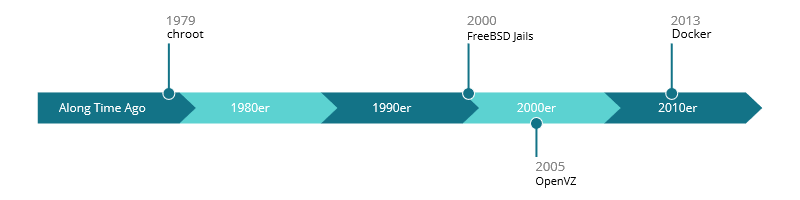
\includegraphics[width=0.8\textwidth]{ZeitContainer.png}
	\end{center}
	\caption[Containertechnologie im Laufe der Zeit]{Containertechnologie im Laufe der Zeit}
	\label{fig:CTZeit}
\end{figure}


\subsection{chroot}
\label{sec:chroot}

Chroot ist ein Befehl, der schon früh in Unix-Systemen eingebaut wurde. Er ermöglicht es einem Prozess ein andres Rootverzeichnis zu geben. Wird in einem Programm \code{chroot()} aufgerufen wechselt es das Verzeichnis und kann nicht auf Dateien außerhalb der zugewiesenen Struktur zugreifen. Diese Abschottung eines Prozess war nie als Sicherheitsfeature vorgesehen und wird hauptsächlich zur Virtualisierung eingesetzt. Mit dem Befehl können einzelne Prozess auf Dateiebene von anderen Anwendungen getrennt werden, weitere Sicherheitsmechanismen oder Isolierungen gibt es nicht.\cite{IEEE7830207,569694, MANPAGE01}

\subsection{OpenVZ}
\label{sec:OpenVZ}

Im Jahr 2005 veröffentlichte die Firma SWsoft (später umbenannt zu Parallels) ihr Projekt OpenVZ unter der GNU GPL Lizenz. OpenVZ basierte auf der Idee der Container ermöglicht es jedoch in jedem Container eine eigene Linux-Distribution auszuführen. Die, durch die Containerumgebung abgegrenzten Betriebssysteme, teilen sich dabei einen Kernel. Dadurch ist der Overhead von OpenVZ deutlich geringer als bei der klassischen Vollvirtualisierung eines Betriebssystems. In den einzelnen Container gibt es jeweils einen eigenen root-User und Dateistruktur, sie können aber unabhängig voneineander gestarten und gestoppt werden. Da sich die Betriebssysteme einen Kernel teilen können auch die Gastsysteme nur Linux-Systeme sein. Da viele der Änderungen von OpenVZ den Kernel von Linux betreffen werden regelmäßig Änderungen von OpenVZ-Patchen in den Kernel von Linux übernommen.\cite{OpenVzNews, IEEE4803091,OpenVzHist}


\subsection{FreeBSD jails}
\label{sec:jails}



\subsection{LXC}
\label{sec:lxc}





\subsection{LXD}
\label{sec:lxd}


\subsection{Solaris Container}
\label{sec:solariscontainer}


\subsection{Windows Containers}
\label{sec:WindowsContainers}

\subsection{Docker}
\label{sec:Docker}

\subsection{Mesos}
\label{sec:Mesos}

\subsection{rkt}
\label{sec:rkt}



